\documentclass[12pt]{article}
\usepackage{graphicx}
\usepackage[dutch]{babel}
\usepackage{amsmath,amsthm,amssymb}
\usepackage{array}
\usepackage[table,xcdraw]{xcolor}
\usepackage{float}
\usepackage[normalem]{ulem}
\usepackage{tcolorbox}
\usepackage{xcolor}
\usepackage[margin=1in]{geometry}
\DeclareMathOperator{\R}{\mathbb{R}}
\DeclareMathOperator{\N}{\mathbb{N}}
\newcommand{\Lim}[1]{\raisebox{0.5ex}{\scalebox{0.8}{$\displaystyle \lim_{#1}\;$}}}
\newcommand{\ols}[1]{\mskip.5\thinmuskip\overline{\mskip-.5\thinmuskip {#1} \mskip-.5\thinmuskip}\mskip.5\thinmuskip}

\title{Temperatuursafhankelijkheid van de soortelijke weerstand van een koperdraad}
\author{Jul Comhaire, Jente Delnoij, Leandro Matthys, Mathias Meersschaut}

\begin{document}
	\maketitle

\section{Theorie}

	\begin{figure}[h]
		\centering
		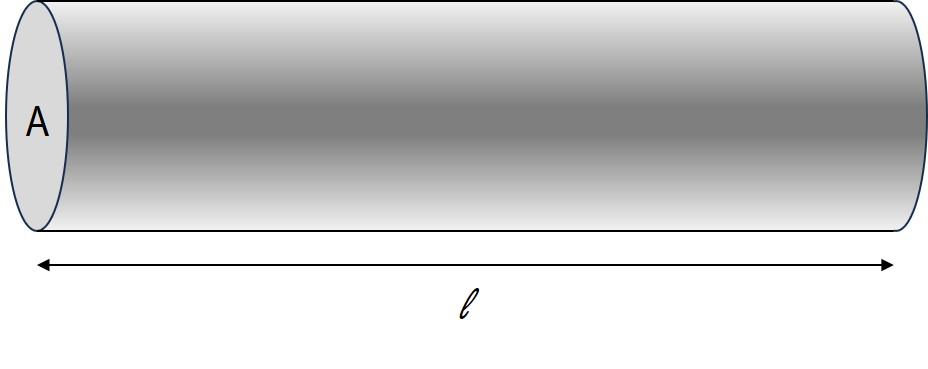
\includegraphics[width=0.5\textwidth]{fig_draad2}
		\caption{Schematische voorstelling van een geleider.}  \label{fig:geleider}
	\end{figure}

	De elektrische weerstand $R$ van een koperdraad  is evenredig met zijn lengte $l$ en omgekeerd evenredig met de dwarsdoorsnede $A$:
		\begin{equation}\label{R}
			R = \rho \frac{l}{A}
		\end{equation}
	Hierin is $\rho$ de soortelijke weerstand uitgedrukt in $\Omega m$. De soortelijke weerstand is afhankelijk van de samenstelling en de puurheid van het materiaal en ook van de temperatuur. Hoe hoger de temperatuur, hoe hoger de weerstand wordt.
	Deze temperatuursafhankelijkheid wordt gegeven \cite{B} door volgende formule:
		\begin{equation}\label{rho}
			\rho(T) = \rho_0 \exp{(\alpha T)}
		\end{equation}
	$\rho_0$ is de soortelijke weerstand van het materiaal bij $0 K$, $\alpha$ is de temperatuurscoëfficiënt van het materiaal (in $K^{-1}$) en $T$ is de absolute temperatuur (in $K$).
	\\
	Voor relatief kleine variaties van de temperatuur \cite{A} kan \eqref{rho} vereenvoudigd worden tot :
		\begin{equation}\label{rho_T}
			\rho(T) = \rho_c [1+\alpha (T-T_c)]
		\end{equation}
	met $T_c$ een referentietemperatuur en $\rho_c$ de soortelijke weerstand bij deze referentietemperatuur. 
	
	In de literatuur \cite{B,C} vinden we dat de soortelijke weerstand van koper bij 20°C (293.15 K) $\rho_{Cu} = 1.75 \, \, 10^{-8} \, \Omega m$ en de temperatuurscoëfficiënt $\alpha = 0.0039 \, K^{-1}$.
	Zo worden \eqref{rho} en \eqref{rho_T} voor koper:
		\begin{equation}\label{rho_cu_exp}
			\rho_{Cu} (T) = 1.75 \, \, 10^{-8}  \exp{(\alpha T)} \, \Omega m  
		\end{equation}
		\begin{equation}\label{rho_cu_approx}
			\rho_{Cu}(T) = 1.75 \, \, 10^{-8} [1+0.0039 (T-293.15)] \, \Omega m     
		\end{equation}
	
\section{Proef}

	Het doel van deze proef is om de temperatuursafhankelijkheid van soortelijke weerstand van koper, $ \rho_{Cu}$, te bepalen.
	Dit doen we door de weerstand $R$ van een kopergeleider op te meten bij verschillende temperaturen. 
	Volgens \eqref{R} geldt immers:
		\begin{equation}\label{rho_ifv_R}
			\rho(T) = R(T) \frac{A}{l}
		\end{equation}
	Omdat $\rho$-waarden van een geleider typisch erg klein zijn (van de orde $10^{-8} \,\Omega m$), kiezen we voor een zo dun mogelijke en lange geleider, zodat de weerstandswaarden binnen het meetbereik van de multimeter vallen.
	\\
	We nemen een koperdraad met een lengte $l=100 \, m$ en een  dwarsdoorsnede $A= 0.8 \, \, 10^{-6} \, m^2$.
	Voor deze specifieke waarden verwachten we een meetbare weerstand:
	$ R = \rho \frac{l}{A}  \approx 10^{-8} \frac{100}{10{^-6}} \, \Omega \approx 1 \, \Omega$.  	
	\textcolor{red}{\\ FYI: bij 20°C zou je dan ongeveer een $R \approx 2.2 \Omega$ moeten vinden.}
	
	De gemeten temperatuurspunten zijn deze van vloeibare stikstof (77 K), droogijs (195 K), temperatuur in diepvriezer (255 K), in frigo (277 K), op kamertemperatuur (293 K) en de temperatuur van kokend water (373 K).
	De weerstand werd opgemeten met een \textcolor{red}{(type/soort)} multimeter in de \textcolor{red}{(gevoeligheid-stand)}-stand. De fout op de meetwaarden kunnen afgeschat worden op \textcolor{red}{$.... \, \Omega$}. Onderstaande tabel toont de meetwaarden.
		\begin{table}[h]
		\centering
		\begin{tabular}{r|l|l}
			T (K) & R ($\Omega$) &  $\rho$ ($10^{-8} \, \Omega m$) \\\hline
		  	 77 &  .... $\pm$ .... &  .... $\pm$ .... \\
			195 &  .... $\pm$ .... &  .... $\pm$ .... \\
			255 &  .... $\pm$ .... &  .... $\pm$ .... \\
			277 &  .... $\pm$ .... &  .... $\pm$ .... \\
			293 &  .... $\pm$ .... &  .... $\pm$ .... \\
			373 &  .... $\pm$ .... &  .... $\pm$ ....  
		\end{tabular}
		\caption{\label{tab:data} Opgemeten weerstand bij 6 verschillende temperaturen en de 	daaruit berekende $\rho_{Cu}$ volgens~\eqref{rho_ifv_R}.}
		\end{table}
	
	De fout op $\rho$ werd als volg berekend:	
	\textcolor{red}{\\foutberekening.}	
	
\section{Analyse}	
	
	\textcolor{red}{Maak hier een plot van $\rho$ ifv $T$: dit zou ca. een rechte moeten geven. (behalve misschien bij 77K en 373 K – zie verder). \\	
	Fit de datapunten met een 1e-graadsfunctie. De richtingscoëfficiënt geeft je dan $\alpha$ (zie eq \eqref{rho_cu_approx}).
	\\ Of fit met  correcte exponent-functie en bepaal zo $\alpha$
	\\ Voeg ook foutberekening op $\alpha$ toe.}
	
	
\section{Discussie}

	\textcolor{red}{Vergelijk de waarde voor $\rho$ bij 293 K met de literatuurwaarde ($\rho_{Cu}(20 ^\circ C) = 1.75 \, \, 10^{-8} \,\Omega m$) en bespreek. \\ Vergelijk ook de gevonden waarde voor de temperatuurscoëfficiënt $\alpha$ met de literatuurwaarde ($\alpha = 0.0039 K^{-1}$) en bespreek.}
	
	We verwachten dat de waarden die we zullen vinden bij $77 \, K$ en $373 \, K$ mogelijks afwijken van lineair verloop, omdat dan (misschien) de benadering van \eqref{rho_cu_exp} door \eqref{rho_cu_approx} niet meer helemaal opgaat. \textcolor{red}{Check dit met de gevonden data. In welk bereik werkt de benadering goed?}
	
	\textcolor{red}{Andere opmerkingen…}


\section{Besluit}

	\textcolor{red}{$\rho(T)$ voor een kopergeleider bepaald. Uit het temperatuursverloop werd vervolgens $\alpha$ bepaald. Blablabla. }
	

\begin{thebibliography}{9}
	
	\bibitem{A} D.C. Giancoli,  \textit{Physics for scientists and Engineers with modern physics},  Pearson Education inc., New York, 2008, p. 658-659.
	
	\bibitem{B} ANONIEM, Soortelijke weerstand, internet, \textit{Wikipedia}, 9 dec 2023, (https://nl.wikipedia.org/wiki/Soortelijke weerstand).
		
	\bibitem{C} R.A. Matula, Electrical resistivity of Copper, Gold, Palladium and Silver, internet, \textit{NIST}, (https://srd.nist.gov/JPCRD/jpcrd155.pdf).
	
\end{thebibliography}



\end{document}